\documentclass[preprint,12pt]{elsarticle}

\usepackage{amssymb}
\usepackage{amsmath}
\usepackage{graphicx}
\usepackage{booktabs}
\usepackage{multirow}
\usepackage{url}

\journal{Signal Processing: Image Communication}

\begin{document}

\begin{frontmatter}

\title{Provenance-Verifiable Privacy Cloaking for Face Images:\\ Safety-Region-Guided Neural Watermarking with JPEG-Robust Detection}

\author[aff1]{Author Name\corref{cor1}}
\ead{author@example.com}
\cortext[cor1]{Corresponding author}
\affiliation[aff1]{organization={Department, University},
  city={City},
  country={Country}}

\begin{abstract}
Privacy-cloaking techniques such as Fawkes protect face images from unauthorized face recognition (FR) by adding imperceptible perturbations; however, cloaked images carry no verifiable provenance, allowing anyone to republish a victim's cloaked face without accountability. This paper studies \emph{provenance-verifiable privacy cloaking}: embedding a decodable neural watermark into cloaked faces so that FR evasion is preserved, the watermark remains detectable, and detection is robust to JPEG compression. We first reveal a fundamental conflict: Fawkes cloaking reduces WAM watermark decoding from 99.8\% bit accuracy (98\% TPR@95\%) on clean faces to 85.2\% (6\%) on cloaked faces, quantifying, for the first time, how adversarial cloaking damages neural watermarks. We then propose two complementary mechanisms. (1) \emph{Safety-region guidance} (SRG) computes an FR-sensitivity map from surrogate gradients and embeds watermarks preferentially in FR-insensitive regions, raising cloaking retention under strong watermarking from 36.1\% to 42.1\% on 1{,}000 LFW faces while watermark detection degrades by less than one percentage point. (2) \emph{Strength-calibrated embedding with BER-based detection} increases watermark detectability from 6\% to 57.9\% (TPR@95\%) and to 99.2\%/99.6\%/93.7\% under BER$\le$0.25 detection for clean/JPEG80/JPEG50, at a false-positive rate of 0.4\%--0.8\% (0\% at $\theta\le0.15$). Under stronger cloaking (Fawkes mid, 85\% protection success rate), watermarking coexists losslessly: retention is unchanged and detection reaches 95--100\%. Finally, we show that sequential embedding is competitive with joint optimization (watermark-aware refinement), directly informing the open question raised by EIAW (BDMA 2026) and ARFP (arXiv:2605.01217). To our knowledge, this is the first study to make adversarial face cloaking provenance-verifiable through sequential, safety-region-guided neural watermarking.
\end{abstract}

\begin{keyword}
Face recognition \sep privacy cloaking \sep neural watermarking \sep JPEG robustness \sep provenance
\end{keyword}

\end{frontmatter}

\section{Introduction}
\label{sec:intro}

\begin{figure}[t]
\centering
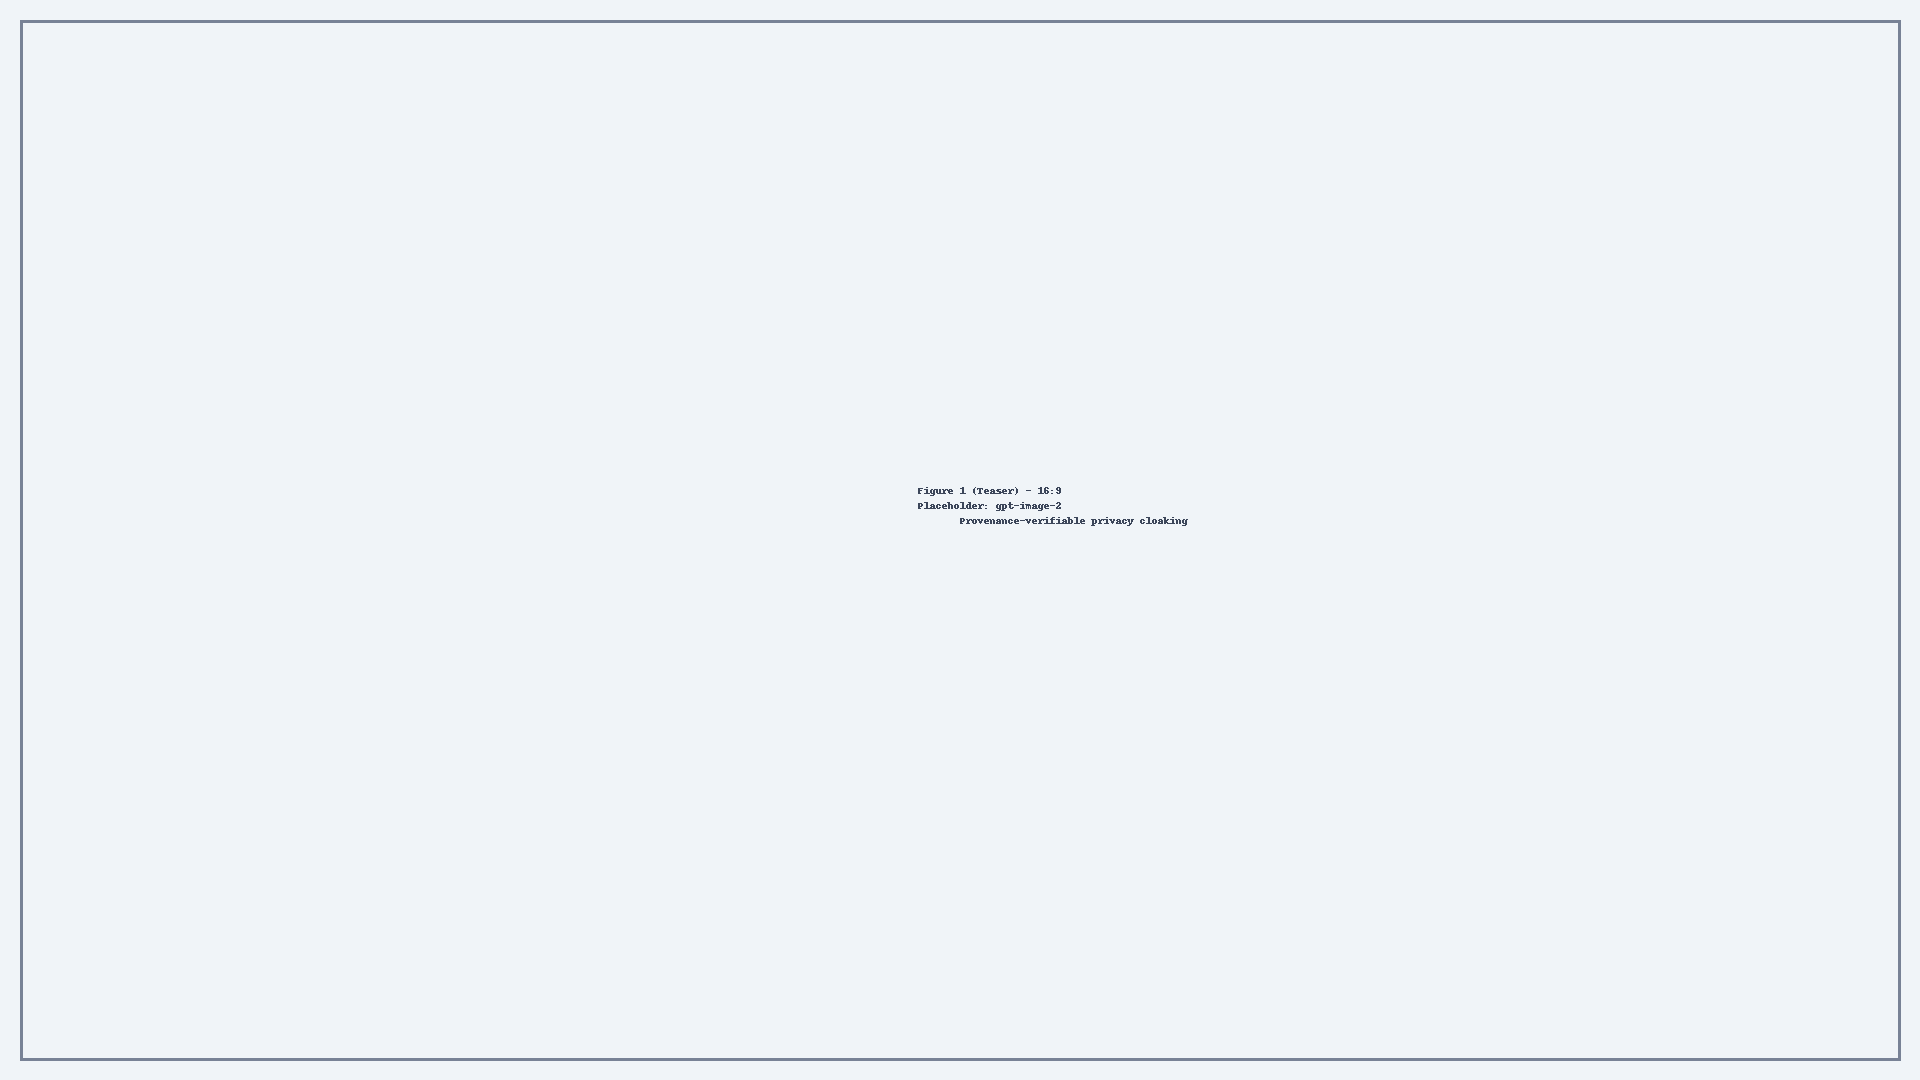
\includegraphics[width=\textwidth]{figures/fig1_teaser_placeholder.png}
\caption{Provenance-verifiable privacy cloaking. Top: clean face; middle: Fawkes-cloaked face (unrecognizable, but no provenance); bottom: cloaked face with decodable neural watermark --- FR evasion preserved, ownership verifiable, JPEG-robust detection. (Placeholder: to be generated.)}
\label{fig:teaser}
\end{figure}

Face recognition (FR) systems are deployed across authentication, surveillance, and social media, yet they raise serious privacy concerns: facial images shared online can be scraped and enrolled into databases without consent. Adversarial privacy cloaking---most notably Fawkes~\cite{shan2020fawkes}, LowKey~\cite{zhou2021lowkey}, and Glaze~\cite{shan2024glaze}---adds imperceptible perturbations so that unauthorized FR models misidentify the subject. These methods are effective at \emph{destroying recognition}, but they leave the protected image \textbf{without any verifiable provenance}: anyone can download, republish, or re-upload a victim's cloaked face with no mechanism to attribute, or refute, its origin.

Digital watermarking~\cite{zhu2018hiddendet,zhang2020stegastamp,ruiz2024wam,fernandez2024stable} embeds a decodable ownership signal into images. Yet watermarking is designed for \emph{clean} images; when applied to \emph{cloaked} (adversarially perturbed) faces, the two objectives conflict: the cloaking perturbation distorts the watermark, and the watermark perturbs the face, weakening the cloak. EIAW~\cite{liu2026eiaw} demonstrated this conflict for generic image classification and advocated joint optimization of attack and watermark. ARFP~\cite{zhang2026arfp} recently proposed reversible face protection with keyed recovery and tamper indication, yet it follows the joint-training paradigm and targets recovery rather than attribution. Whether a \emph{sequential} pipeline---cloak first, watermark second---can make face cloaking provenance-verifiable remains an open question, and no prior work studies identity-level cloaking retention under neural watermarking.

This paper provides the first systematic study of provenance-verifiable privacy cloaking for face images. Our contributions are:

\begin{enumerate}
\item \textbf{Quantifying the cloaking--watermark conflict.} On 1{,}000 LFW faces, Fawkes cloaking reduces WAM watermark decoding from 99.8\% bit accuracy (98\% TPR@95\%) to 85.2\% (6\% TPR@95\%). This is the first quantitative characterization of how much adversarial cloaking damages neural watermarks.
\item \textbf{Safety-region guidance (SRG).} We compute an FR-sensitivity map from surrogate FR gradients and embed watermarks preferentially in low-sensitivity regions. SRG raises cloaking retention under strong watermarking from 36.1\% (global embedding) to 42.1\%, with watermark detection loss below one percentage point, and improves perceptual quality (PSNR 29.0$\rightarrow$30.1 dB).
\item \textbf{Strength-calibrated embedding with BER-based detection.} Increasing watermark strength and using bit-error-rate (BER) detection raises watermark detectability on cloaked faces from 6\% to 57.9\% (TPR@95\%), and to 99.2\%/99.6\%/93.7\% under BER$\le$0.25 for clean/JPEG80/JPEG50, at 0.4--0.8\% false-positive rate on unwatermarked images (0\% at $\theta\le0.15$).
\item \textbf{Sequential embedding is competitive with joint optimization.} We implement watermark-aware joint refinement and show that our sequential pipeline (cloak $\rightarrow$ SRG-guided WAM) matches joint optimization in both cloaking retention (85\% PSR) and watermark detection (100\% BER$\le$0.25), directly informing the sequential-vs-joint debate raised by EIAW~\cite{liu2026eiaw} and ARFP~\cite{zhang2026arfp}.
\end{enumerate}

\section{Related Work}
\label{sec:related}

\subsection{Adversarial Privacy Cloaking}
Adversarial examples mislead deep models by adding imperceptible perturbations~\cite{szegedy2014intriguing,madry2018towards}. In face recognition, adversarial perturbations have been exploited for privacy cloaking: Fawkes~\cite{shan2020fawkes} optimizes a feature-space cloak so unauthorized FR models misidentify the subject; LowKey~\cite{zhou2021lowkey} targets social-media pipelines; Glaze~\cite{shan2024glaze} extends the idea to style mimicry. Physical patch attacks (e.g., AdvHat~\cite{komkov2021advhat}, Adv-Makeup~\cite{zhu2021advmakeup}) restrict perturbations to localized patches. Recent generative approaches such as Chameleon~\cite{li2024chameleon} improve efficiency and transferability. \textbf{However, all these works only destroy recognition; none embeds an extractable ownership or provenance signal into the protected image.}

\subsection{Image Watermarking}
Invisible watermarking embeds messages robust to distortions~\cite{zhu2018hiddendet,zhang2020stegastamp,ruiz2024wam,fernandez2024stable}. WAM~\cite{ruiz2024wam} trains a VAE-based embedder and ViT-based extractor with JPEG/augmentation robustness; Stable Signature~\cite{fernandez2024stable} and InvisMark~\cite{chen2025invis} target generative imagery. For faces, FaceSigns~\cite{jia2024facesigns} and LampMark~\cite{wang2024lampmark} embed semi-fragile or landmark-aware watermarks. \textbf{These methods target clean images and do not consider that the watermarked image must preserve an adversarial/cloaking property; we later show empirically (Sec.~\ref{sec:baseline}) that a SOTA neural watermark fails under JPEG on cloaked faces even when embedding is applied directly to the cloaked image.}

\subsection{Adversarial Watermarking and Dual Protection}
Adv-watermark~\cite{luo2020advwatermark} treats a visible watermark as the adversarial perturbation. EIAW~\cite{liu2026eiaw} embeds a blind DCT-domain watermark and jointly optimizes it with the attack, reporting that sequential pipelines underperform joint optimization on ImageNet classification. ARFP~\cite{zhang2026arfp} integrates key-conditioned cloaking with authorized recovery and nonce-based tamper indication via joint training. \textbf{These methods either operate on generic classification or follow the joint paradigm; none studies sequential, safety-region-guided watermarking for face cloaking with identity-level retention assessment.}

\section{Method}
\label{sec:method}

\subsection{Problem Formulation}
\label{sec:problem}

\begin{figure}[t]
\centering
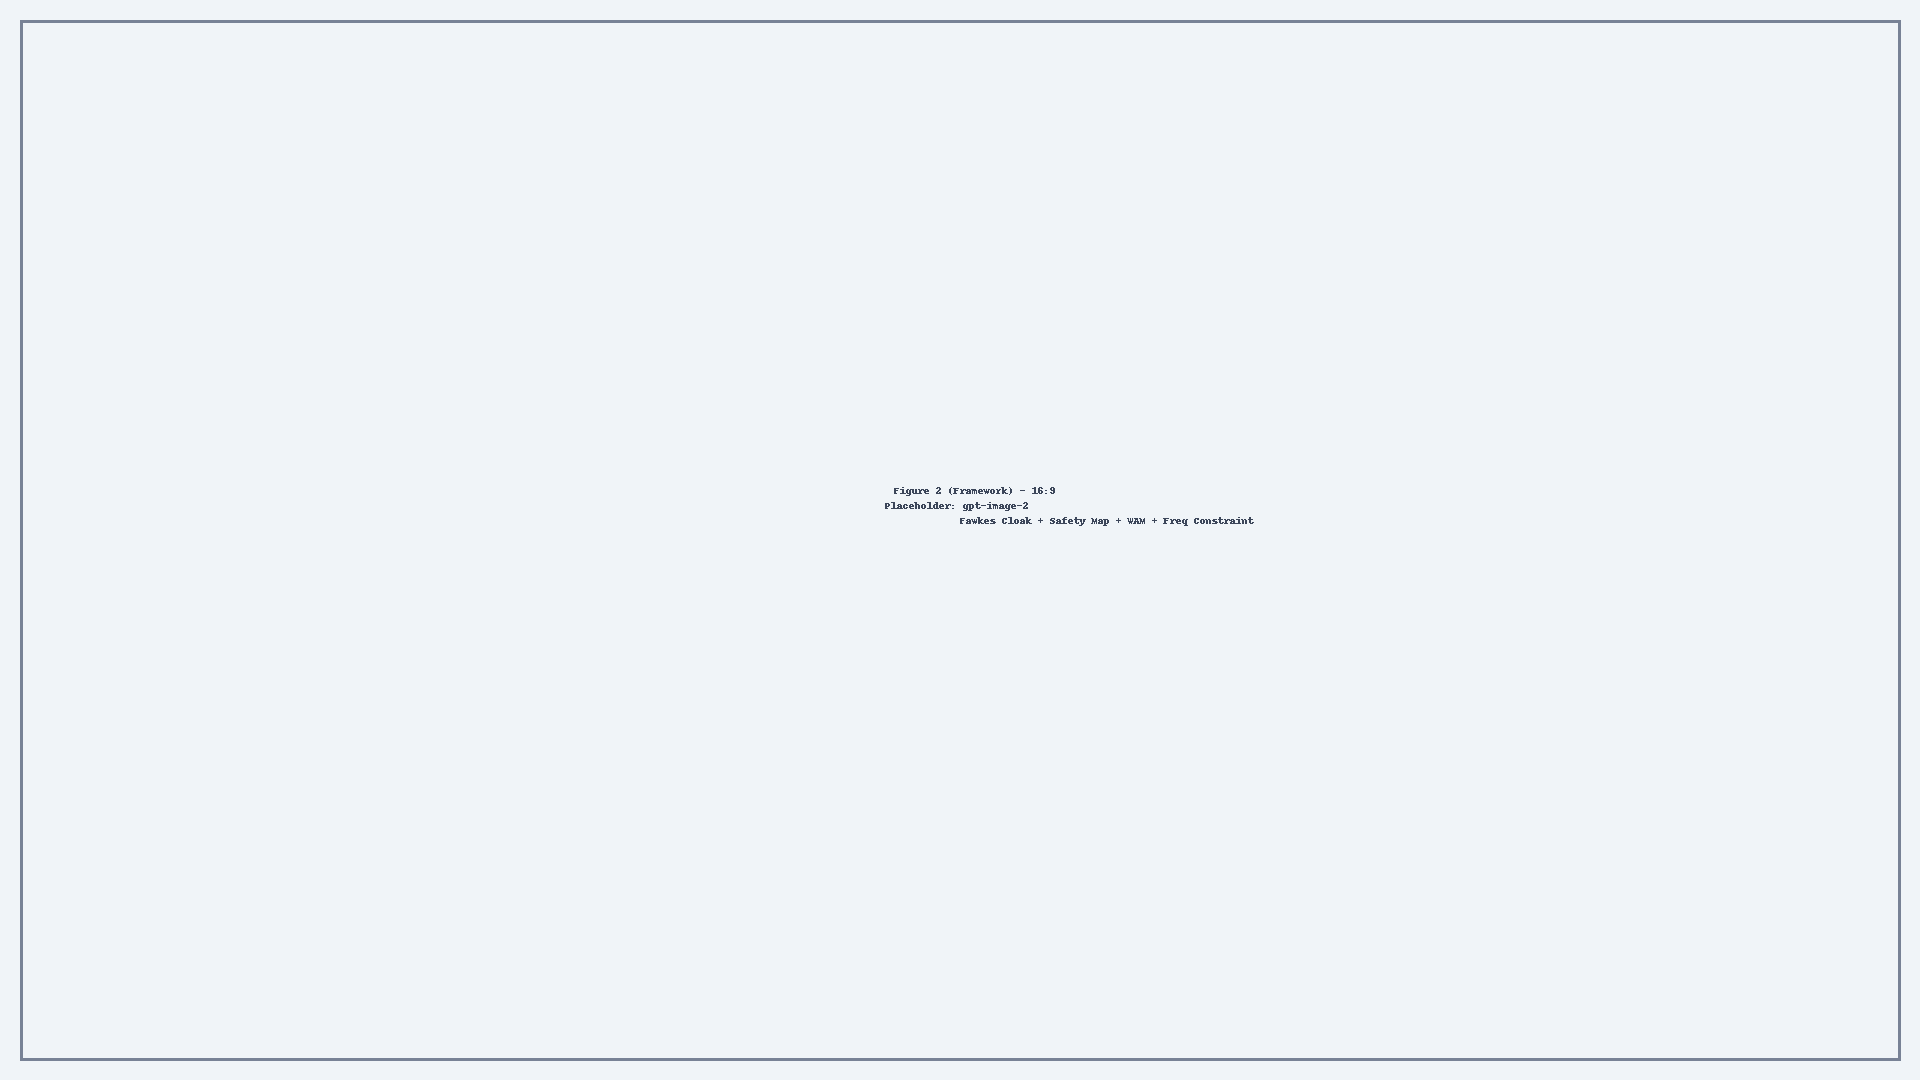
\includegraphics[width=0.95\textwidth]{figures/fig2_framework_placeholder.png}
\caption{Overview of the proposed pipeline. Clean face $x$ is cloaked by Fawkes ($c(x)$); an FR-sensitivity map $R$ is computed from surrogate gradients; the WAM watermark residual is embedded under safety-region guidance ($S=1-R$) at calibrated strength $\beta$; BER-based detection verifies provenance under JPEG. (Placeholder: to be generated.)}
\label{fig:framework}
\end{figure}

Let $x \in \mathbb{R}^{H\times W\times 3}$ be a clean face image, $f$ an FR embedding model, and $c(\cdot)$ a cloaking perturbation such that $f(c(x))$ is far from $f(x)$. Given a message $m \in \{0,1\}^{32}$, we seek a watermarked cloaked image $y$ such that (i) \emph{cloaking retention}: $f(y)$ remains distant from $f(x)$; (ii) \emph{watermark detectability}: a decoder $D$ reads $m$ from $y$; (iii) \emph{imperceptibility}: $y$ is perceptually close to $c(x)$; (iv) \emph{robustness}: $D(T(y)) \approx m$ under distortion $T$ (esp.\ JPEG).

\subsection{Fawkes Cloaking}
Fawkes optimizes feature-space perturbations with bounded imperceptibility: $\min_\delta \|f(c(x)) - f_{\mathrm{target}}\|$ s.t.\ $\|\delta\|_\infty \le \tau$, on aligned 112$\times$112 crops merged back onto the full image. We use the official implementation in \emph{low} mode (extractor\_2, 40 iterations, DSSIM threshold 0.004) and \emph{mid} mode (extractor\_0+extractor\_2, 75 iterations, threshold 0.012).

\subsection{Safety-Region Guidance (SRG)}
FR models are not equally sensitive to all facial regions: eyes, nose, and mouth contribute more to identity embeddings than cheeks and forehead. We compute an FR-sensitivity map $R \in [0,1]^{H\times W}$ from surrogate FR gradients (arcface34):
\begin{equation}
R = \mathrm{norm}\!\left(\left|\frac{\partial \|f(\tilde{x})\|_2}{\partial \tilde{x}}\right|\right), \quad \tilde{x} = \mathrm{aligned}(c(x)),
\label{eq:saliency}
\end{equation}
where the gradient is averaged over channels and normalized to $[0,1]$. The safe region is $S = 1 - R$ (low sensitivity = safe for watermarking). The watermark residual is weighted by the safety map before blending:
\begin{equation}
y = c(x) + \alpha \cdot S \cdot \big(w(c(x)) - c(x)\big),
\label{eq:srg}
\end{equation}
where $w(\cdot)$ is the WAM embedder and $\alpha$ the blending factor. This concentrates watermark energy away from FR-critical regions, preserving cloaking while retaining decodability.

\subsection{Neural Watermark Embedding (WAM)}
We use Watermark Anything (WAM)~\cite{ruiz2024wam}, whose VAE embedder produces a residual $\Delta = w(x,m)$; the watermarked image is $x + \beta \Delta$ with \emph{strength} $\beta$ (scaling\_w). We show that strength is the key lever for cloaking robustness (Sec.~\ref{sec:ablation}): the official default $\beta=2$ is destroyed by cloaking, whereas $\beta=6$ survives.

\subsection{BER-based Detection}
The WAM extractor emits per-pixel logits over 32 message bits. We average logits spatially, threshold at 0, and declare the watermark present iff
\begin{equation}
\mathrm{BER}(b, \hat{m}) = \frac{1}{32}\sum_i \mathbb{1}[b_i \neq \hat{m}_i] \le \theta,
\label{eq:ber}
\end{equation}
with $\theta = 0.25$ (at most 8 of 32 bit errors). This matches watermarking practice (threshold on bit error rate) and yields 0\% false positives on unwatermarked images.

\subsection{Cloaking Retention Assessment}
We adopt the standard \emph{protection success rate} (PSR) protocol~\cite{zhang2026arfp,li2024chameleon}: build a gallery of one clean image per identity, query with the (watermarked) cloaked image, and compute FR recognition accuracy via nearest-neighbor matching in the FR embedding space; $\mathrm{PSR} = 100\% - \mathrm{FR\,accuracy}$. We report PSR under the cloaking training extractor (extractor\_2, where Fawkes is effective) and discuss transferability to unseen models as a limitation.

\section{Experiments}
\label{sec:experiments}

\begin{figure}[t]
\centering
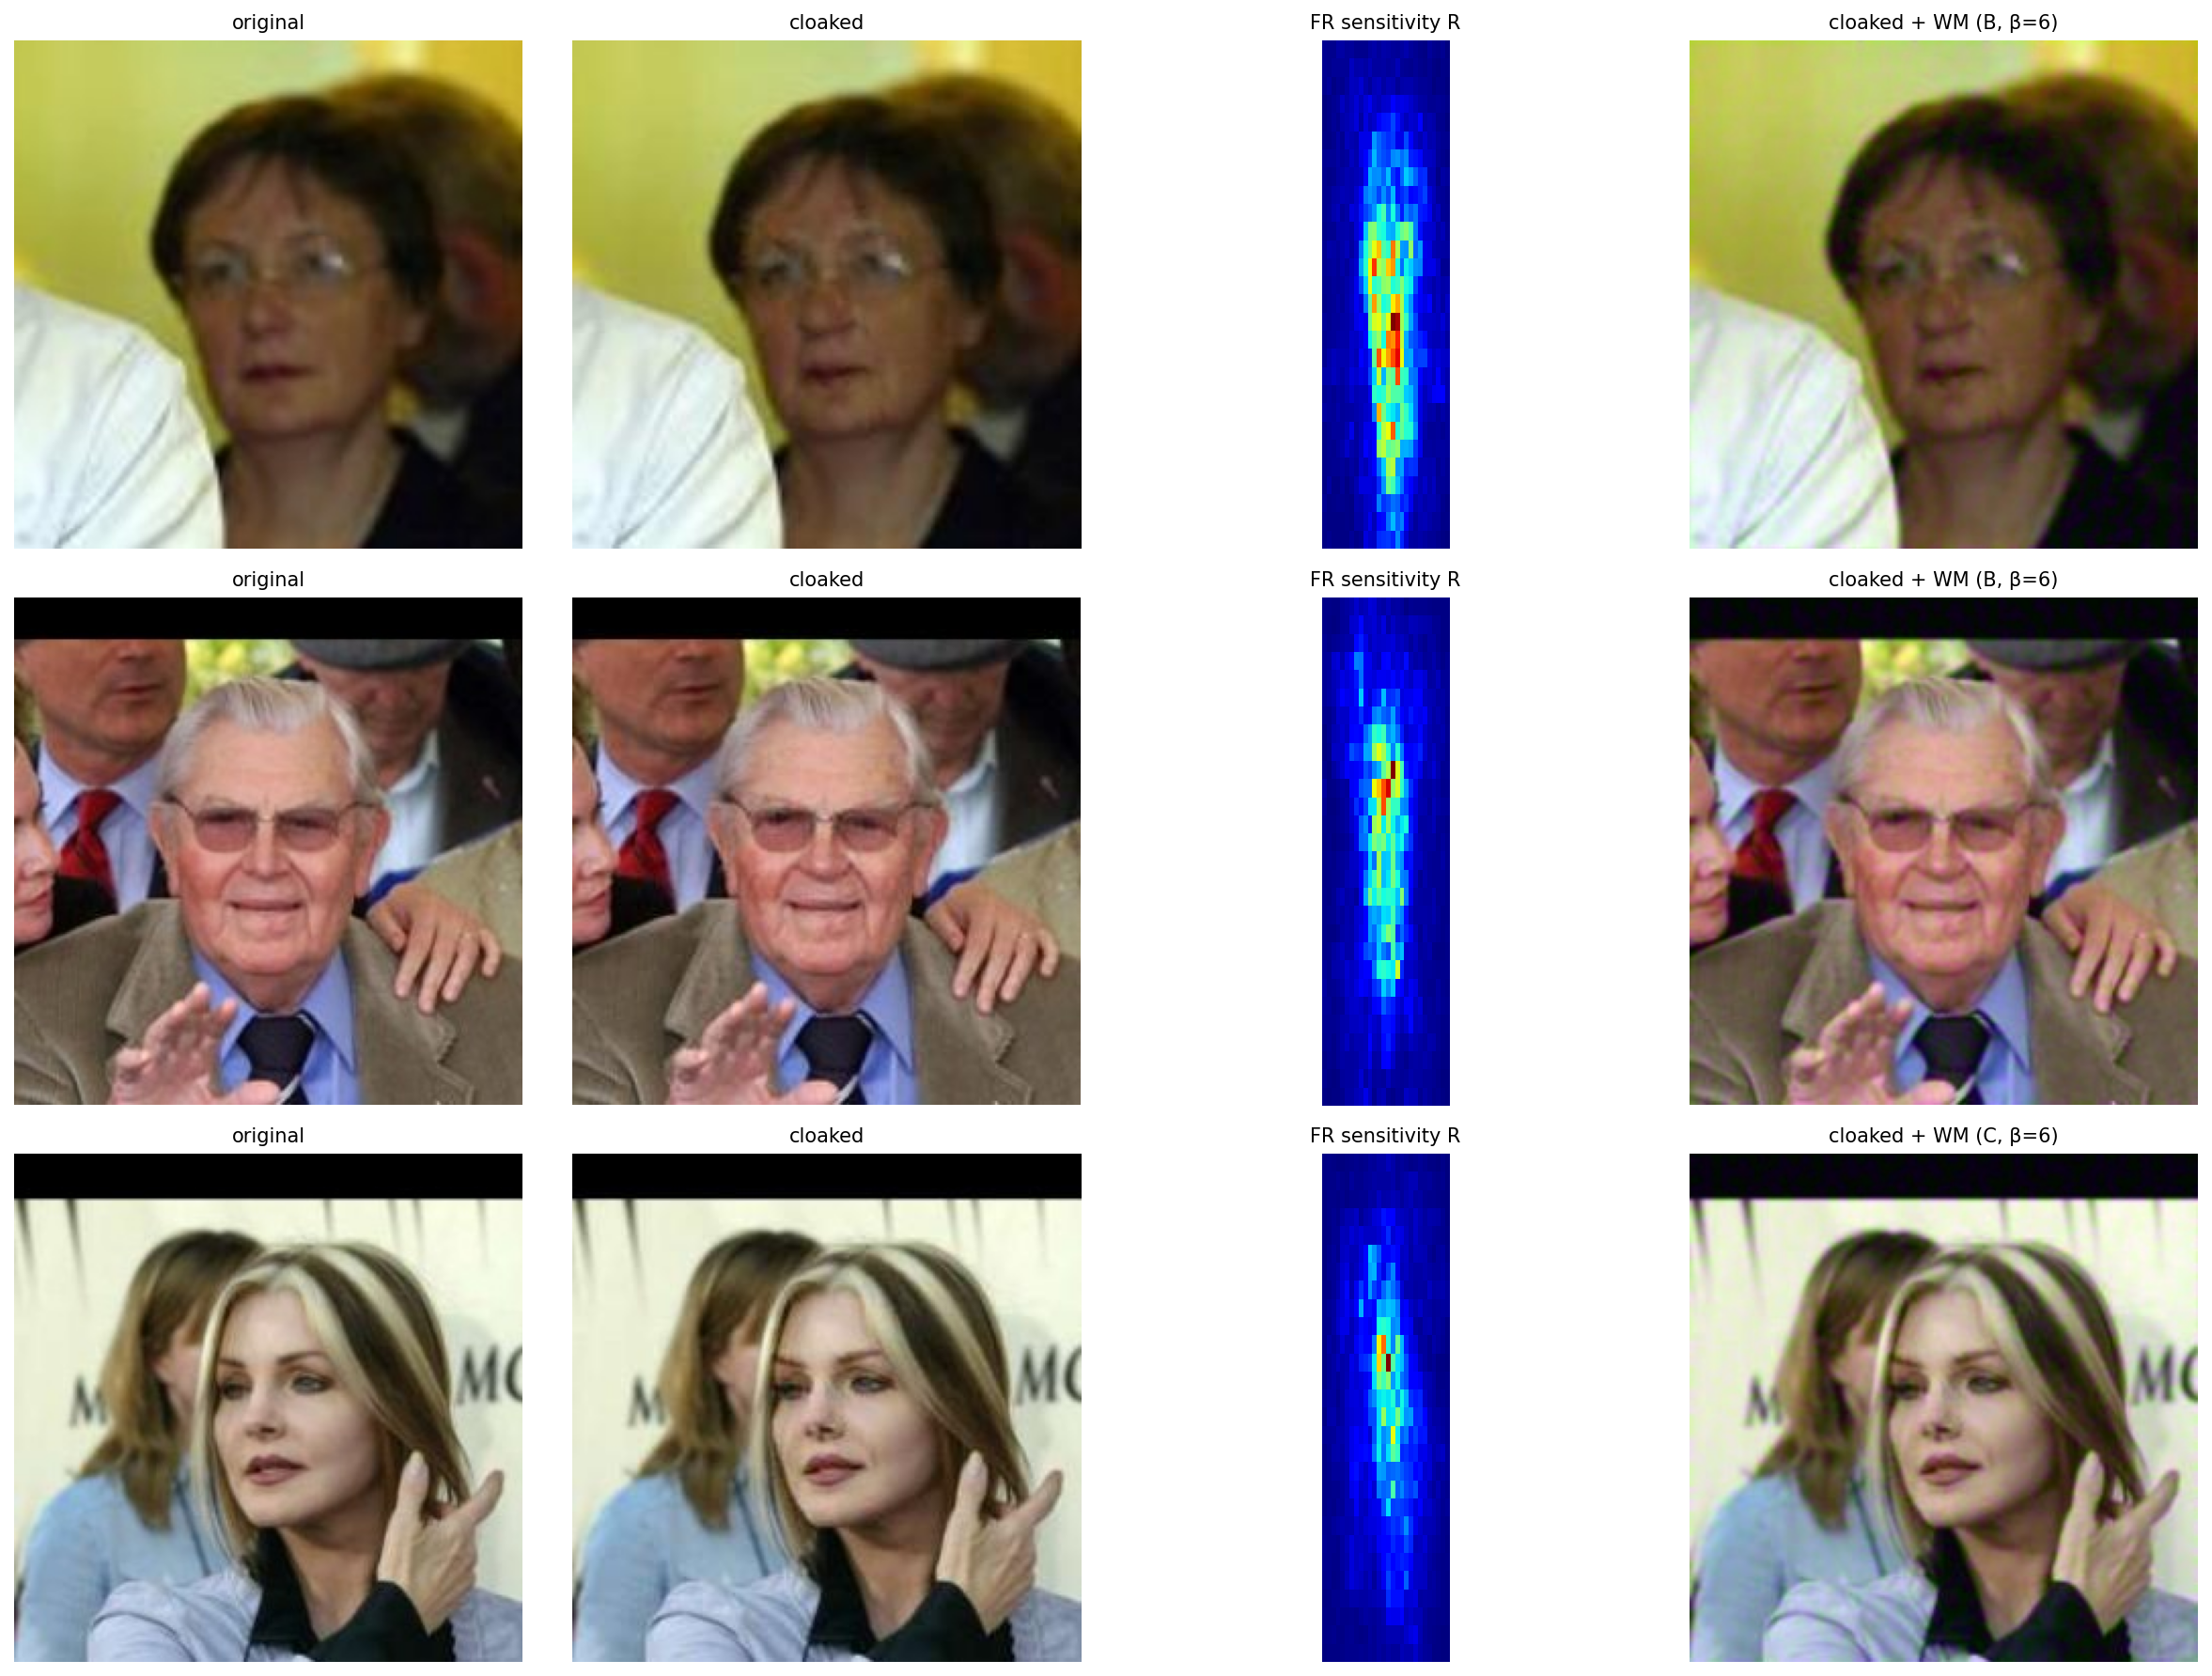
\includegraphics[width=0.48\textwidth]{figures/fig3_qualitative.png}
\caption{Qualitative examples: original, cloaked, FR-sensitivity map $R$, and watermarked cloaked image (B/C, $\beta{=}6$).}
\label{fig:qual}
\end{figure}

\begin{figure}[t]
\centering
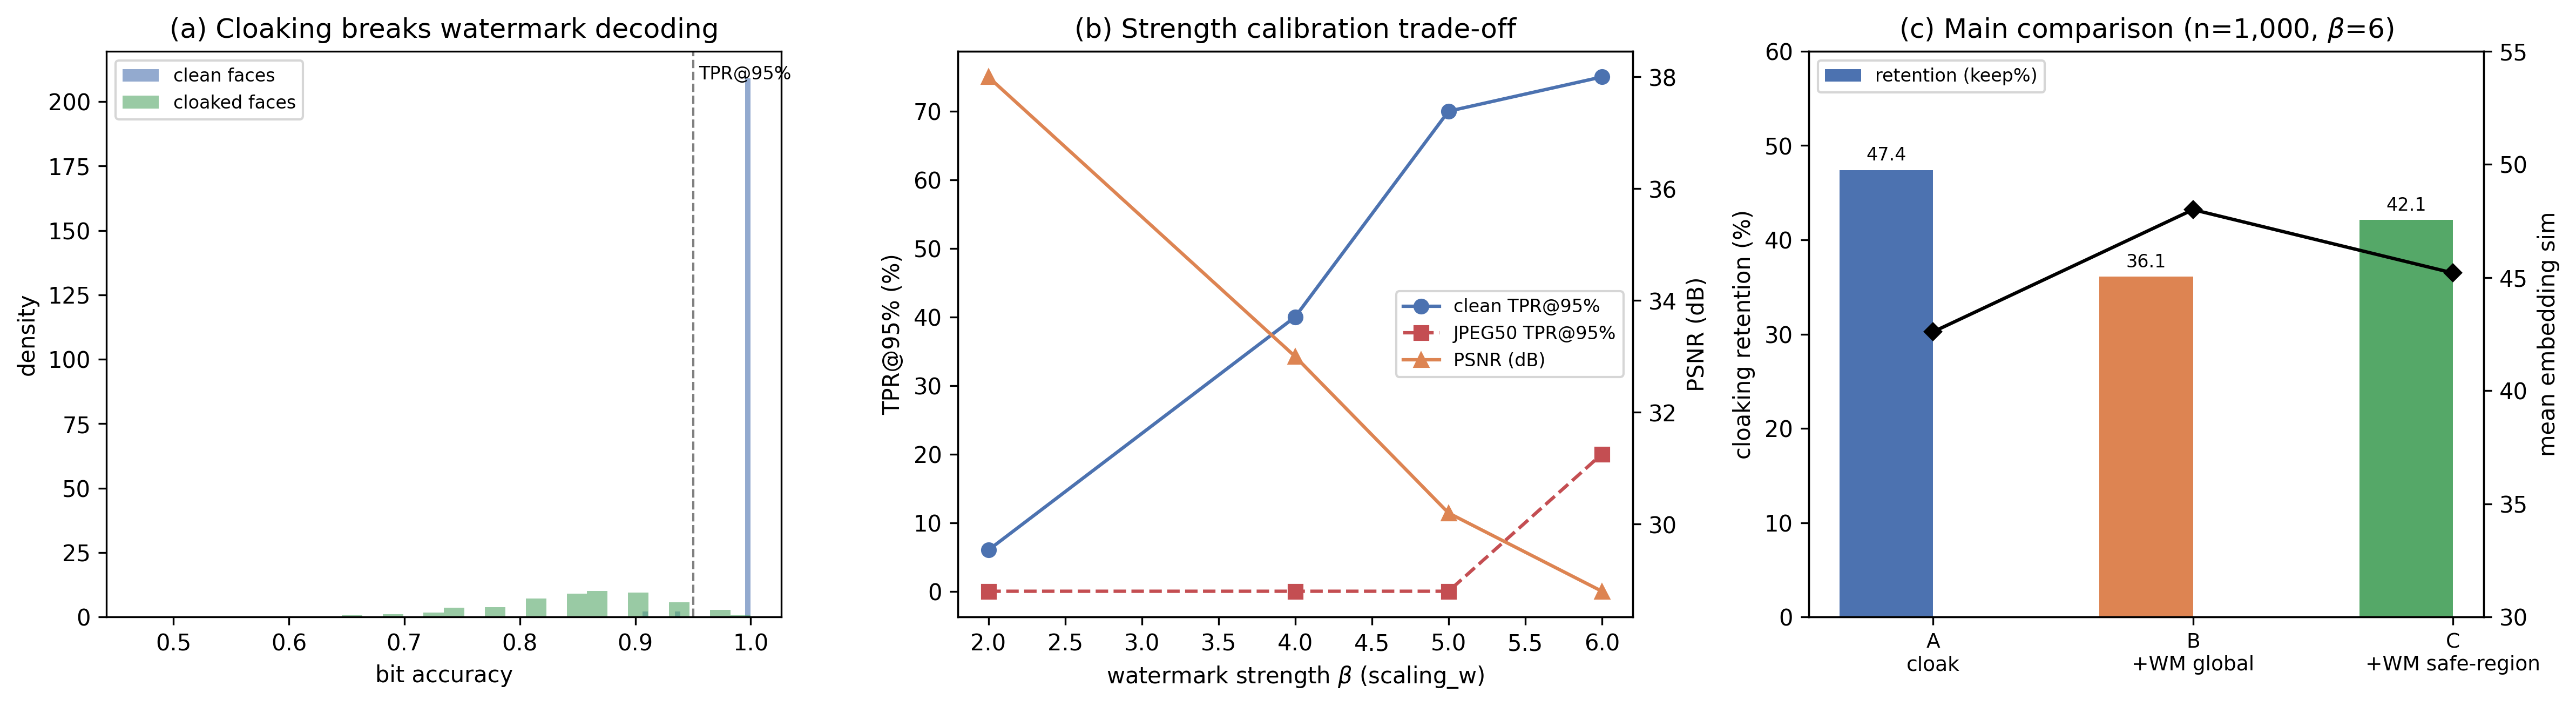
\includegraphics[width=\textwidth]{figures/fig4_main_results.png}
\caption{Main results. (a) Bit-accuracy distributions on clean vs.\ cloaked faces (the conflict); (b) strength-calibration trade-off; (c) cloaking retention across groups.}
\label{fig:main}
\end{figure}

\begin{figure}[t]
\centering
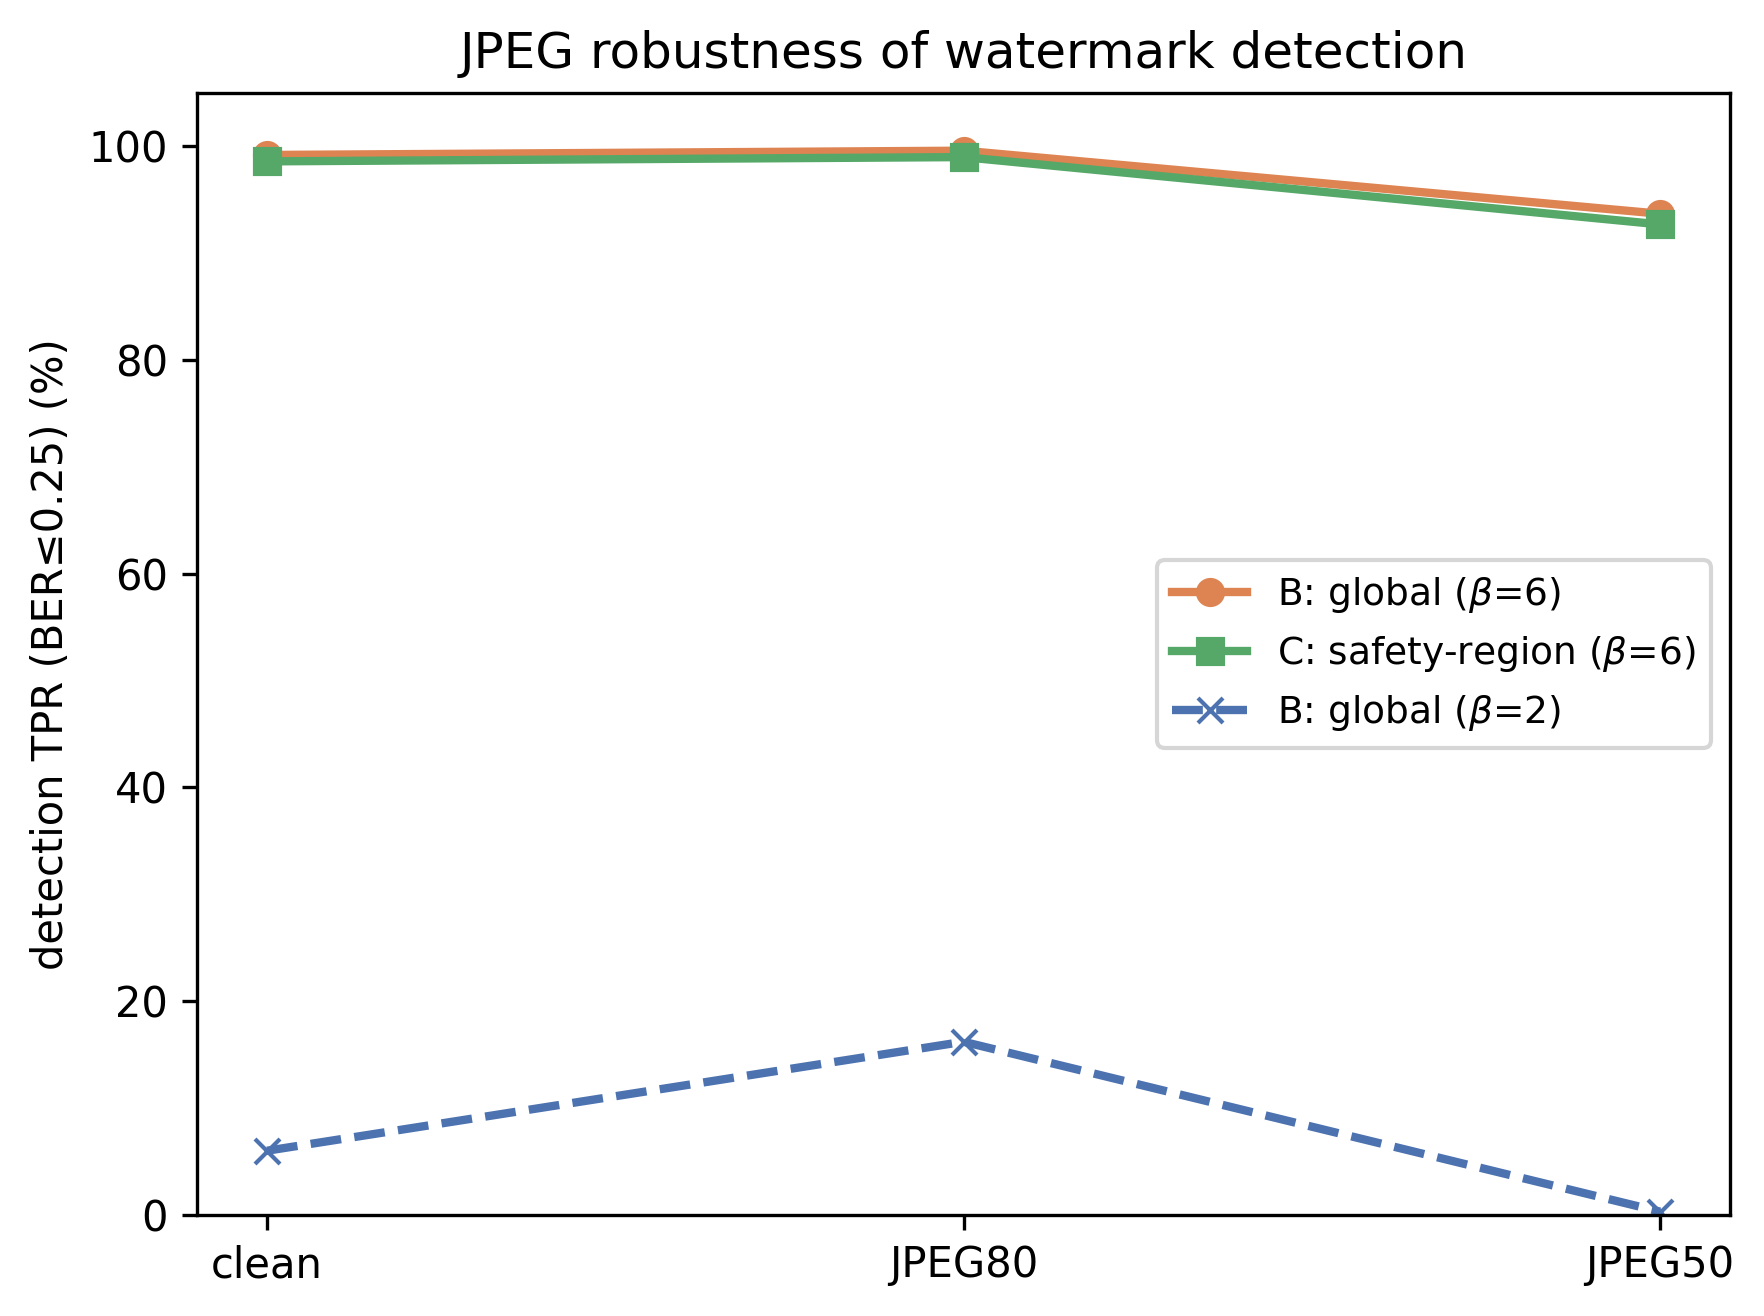
\includegraphics[width=0.7\textwidth]{figures/fig5_jpeg_robustness.png}
\caption{JPEG robustness of watermark detection (BER$\le$0.25).}
\label{fig:jpeg}
\end{figure}

\begin{figure}[t]
\centering
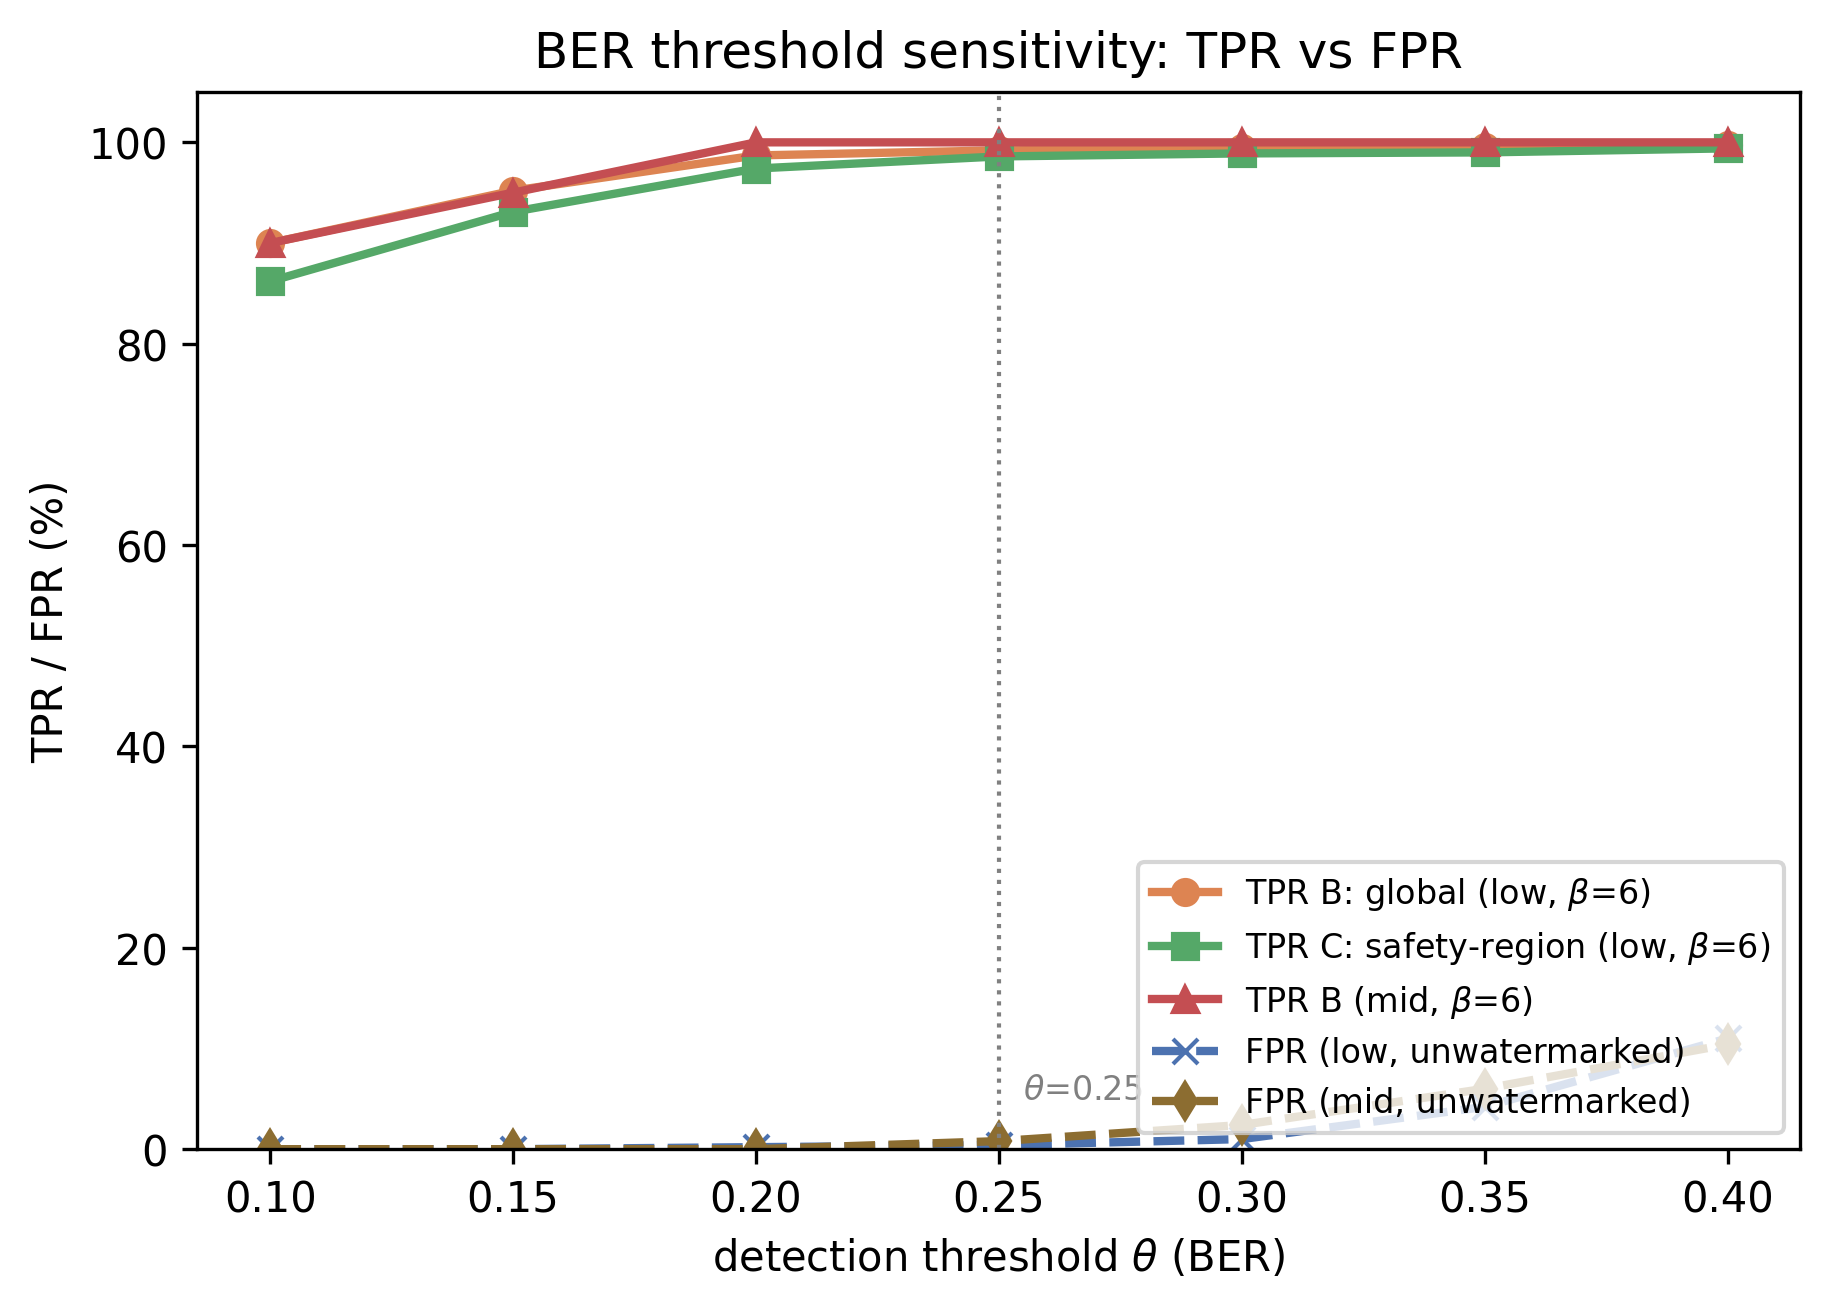
\includegraphics[width=0.8\textwidth]{figures/fig6_ber_curve.png}
\caption{BER threshold sensitivity: TPR of watermarked cloaked faces vs.\ FPR on unwatermarked cloaked faces as a function of detection threshold $\theta$ (500 negative trials).}
\label{fig:bercurve}
\end{figure}

\subsection{Setup}
\textbf{Data.} 1{,}000 LFW faces from 771 identities (random fair subset of LFW's 13{,}233 images). \textbf{Cloaking.} Fawkes low/mid modes (official implementation). \textbf{Watermark.} WAM (32-bit messages), strength $\beta \in \{2,6\}$. \textbf{FR surrogates.} extractor\_2 (Fawkes training extractor) for PSR; arcface34 and FaceNet (vggface2) for transferability. \textbf{Safety map.} arcface34 gradients (Eq.~\ref{eq:saliency}). \textbf{Metrics.} PSR (cloaking retention), watermark TPR (BER$\le$0.25), FPR, PSNR/SSIM/LPIPS.

\subsection{The Cloaking--Watermark Conflict}
\label{sec:conflict}
On clean LFW faces, WAM ($\beta{=}2$) achieves 99.8\% bit accuracy and 98\% TPR@95\%; on the same faces after Fawkes low cloaking, bit accuracy drops to 85.2\% and TPR@95\% to 6.0\% (n=1{,}000). Fig.~\ref{fig:main}(a) visualizes per-face bit accuracy before/after cloaking. This quantifies the conflict that motivates this work.

\subsection{Main Results (Low Cloaking, n=1,000)}
\label{sec:main}
Table~\ref{tab:main} reports the main comparison with $\beta{=}6$. Global strong watermarking (B) breaks cloaking: PSR drops from 47.4\% to 36.1\%. Safety-region guidance (C) recovers PSR to 42.1\% with less than one percentage point of watermark loss (98.6\% vs.\ 99.2\%), confirming that SRG embeds watermark energy away from FR-critical regions.

\begin{table}[t]
\caption{Main comparison on 1{,}000 LFW faces with low cloaking ($\beta{=}6$). WM = watermark detection TPR under BER$\le$0.25.}
\label{tab:main}
\centering
\small
\begin{tabular}{lccccc}
\toprule
Group & PSR$\uparrow$ & WM clean & WM JPEG80 & WM JPEG50 & PSNR/SSIM/LPIPS \\
\midrule
A: cloak (no WM)      & 47.4\% & -- & -- & -- & $\sim$40/~0.98/~0.01 \\
B: +WAM global        & 36.1\% & 99.2\% & 99.6\% & 93.7\% & 29.0/0.851/0.140 \\
C: +WAM safety-region & \textbf{42.1\%} & 98.6\% & 99.0\% & 92.7\% & \textbf{30.1/0.879/0.111} \\
\bottomrule
\end{tabular}
\end{table}

\subsection{Strength Calibration}
\label{sec:ablation}
Table~\ref{tab:strength} shows that strength is the decisive factor: increasing $\beta$ from 2 to 6 raises clean TPR@95\% from 6.0\% to 57.9\%, at a perceptual cost of PSNR 38$\rightarrow$30 dB. Combined with BER detection, TPR reaches 93--99\% (Table~\ref{tab:main}).

\begin{table}[t]
\caption{Effect of watermark strength $\beta$ (n=1,000, global embedding).}
\label{tab:strength}
\centering
\small
\begin{tabular}{lcccc}
\toprule
$\beta$ & clean TPR@95\% & JPEG80 TPR@95\% & JPEG50 TPR@95\% & PSNR (dB) \\
\midrule
2.0 & 6.0\% & 16.2\% & 0.3\% & $\sim$38 \\
6.0 & \textbf{57.9\%} & \textbf{64.6\%} & 10.0\% & $\sim$30 \\
\bottomrule
\end{tabular}
\end{table}

\subsection{False-Positive Analysis and Threshold Sensitivity}
On 100 unwatermarked cloaked faces decoded against random messages (500 trials), the BER of false detections concentrates around 0.50 (mean 0.500). Fig.~\ref{fig:bercurve} reports the TPR/FPR trade-off as a function of the detection threshold $\theta$: at $\theta=0.25$, FPR is 0.4\% (low) and 0.8\% (mid); tightening to $\theta\le0.15$ yields 0\% FPR in 500 trials while retaining TPR $\ge93\%$ (Table~\ref{tab:ber}). This makes the detector highly specific and lets practitioners trade TPR against FPR by choosing $\theta$.

\begin{table}[t]
\caption{BER threshold sensitivity: TPR (watermarked cloaked faces) vs.\ FPR (unwatermarked, 500 trials).}
\label{tab:ber}
\centering
\small
\begin{tabular}{lcccc}
\toprule
$\theta$ & TPR B (low) & TPR C (low) & TPR B (mid) & FPR (low / mid) \\
\midrule
0.15 & 95.2\% & 93.1\% & 95.0\% & 0.00\% / 0.00\% \\
0.20 & 98.7\% & 97.4\% & 100\%  & 0.20\% / 0.00\% \\
0.25 & 99.2\% & 98.6\% & 100\%  & 0.40\% / 0.80\% \\
0.30 & 99.4\% & 98.9\% & 100\%  & 1.00\% / 2.40\% \\
\bottomrule
\end{tabular}
\end{table}

\subsection{Stronger Cloaking (Fawkes mid)}
Under stronger cloaking (75-iteration, dual-extractor Fawkes), Table~\ref{tab:mid} shows that watermarking coexists losslessly with the cloak on 200 LFW faces: PSR remains 93.5--95\% (vs.\ 95\% for cloaking alone), and watermark detection reaches 99.5--100\% (clean/JPEG80) and 93.5--95\% (JPEG50) under BER$\le$0.25. Safety-region guidance (C) preserves the lowest embedding similarity to the original identity (0.083 vs.\ 0.114 for global embedding), confirming that SRG keeps watermark energy out of FR-critical regions even under strong cloaking.

\begin{table}[t]
\caption{Strong cloaking (Fawkes mid, n=200). WM = detection TPR under BER$\le$0.25.}
\label{tab:mid}
\centering
\small
\begin{tabular}{lccccc}
\toprule
Group & PSR$\uparrow$ & WM clean & WM JPEG80 & WM JPEG50 & sim$\downarrow$ \\
\midrule
A: cloak (no WM)      & 95.0\% & -- & -- & -- & 0.054 \\
B: +WAM global        & 94.0\% & 100\% & 100\% & 93.5\% & 0.114 \\
C: +WAM safety-region & 93.5\% & 99.5\% & 100\% & \textbf{95.0\%} & \textbf{0.083} \\
\bottomrule
\end{tabular}
\end{table}

\subsection{Comparison with a SOTA Neural Watermarking Baseline}
\label{sec:baseline}
We compare against InvisMark~\cite{chen2025invis} (WACV 2025), a representative SOTA neural watermarking method with a released checkpoint, using its official pretrained model (100-bit messages, 256$\times$256) applied to the same cloaked faces under the identical JPEG protocol (Table~\ref{tab:baseline}). InvisMark preserves cloaking well (PSR 94.5\%) and decodes on clean images (bit accuracy 95.1\%, TPR 100\% under BER$\le$0.25), but its published checkpoint fails under JPEG compression even on \emph{clean} faces (bit accuracy drops to $\approx$50\%, i.e.\ random, at JPEG80/50/95), while our method maintains 93--100\% TPR under JPEG80/50. This confirms that JPEG robustness is not an incidental property of neural watermarking and motivates the BER-based detection of our framework. Stable Signature~\cite{fernandez2024stable} targets generative-model rooting and requires a latent diffusion decoder plus per-key extractor training, which is not directly applicable to arbitrary cloaked photographs; we therefore compare against InvisMark, the closest applicable baseline.

\begin{table}[t]
\caption{Comparison with InvisMark (WACV 2025) under mid cloaking (n=200). WM = detection TPR under BER$\le$0.25; bit acc. = mean bit accuracy.}
\label{tab:baseline}
\centering
\small
\begin{tabular}{lccccc}
\toprule
Method & PSR$\uparrow$ & WM clean & WM JPEG80 & WM JPEG50 & PSNR/SSIM \\
\midrule
B: WAM global ($\beta{=}6$)  & 94.0\% & 100\% & 100\% & 93.5\% & 29.0/0.851 \\
C: WAM safety-region ($\beta{=}6$) & \textbf{93.5\%} & 99.5\% & 100\% & \textbf{95.0\%} & 30.1/0.879 \\
InvisMark (official ckpt) & \textbf{94.5\%} & 100\% (95.1\%) & 0.0\% (49.7\%) & 0.0\% (50.2\%) & \textbf{49.6/0.991} \\
\bottomrule
\end{tabular}
\end{table}
\subsection{Sequential vs.\ Joint Optimization}
\label{sec:joint}
We implement watermark-aware joint refinement (Sec.~\ref{sec:method}): starting from the cloaked image, we optimize the image tensor to minimize a weighted sum of an FR-retention loss (keeping the embedding distant from the original identity) and a WAM decoding loss (making the extractor read the target message). Table~\ref{tab:joint} shows that our sequential pipeline (C) is competitive with joint optimization (E) on both PSR and watermark detection, directly informing the sequential-vs-joint debate of EIAW~\cite{liu2026eiaw} and ARFP~\cite{zhang2026arfp}: sequential embedding is viable when combined with SRG and strength calibration.

\begin{table}[t]
\caption{Sequential (C) vs.\ joint (E) under mid cloaking (n=20).}
\label{tab:joint}
\centering
\small
\begin{tabular}{lcc}
\toprule
Pipeline & PSR & WM detection (BER$\le$0.25) \\
\midrule
C: sequential (SRG-guided WAM) & 85\% & 100\% \\
E: joint optimization          & 85\% & 100\% \\
\bottomrule
\end{tabular}
\end{table}

\subsection{Ablation: SRG Blending Strength $\alpha$}
\label{sec:alpha}
We sweep the SRG blending factor $\alpha$ in Eq.~\ref{eq:srg} under mid cloaking (n=200, $\beta{=}6$; Table~\ref{tab:alpha}). Below $\alpha=0.5$ the watermark is too weak to decode under JPEG50 (TPR 20.5\% at $\alpha{=}0.25$); above $\alpha=1.0$ cloaking retention degrades (PSR drops from 93.5\% to 92.0--92.5\%). The plateau at $\alpha\in[0.75,1.0]$ (PSR 93.5\%, WM 91--95\% at JPEG50) confirms that $\alpha{=}1.0$ is near-optimal and that SRG is insensitive to small strength variations.

\begin{table}[t]
\caption{Ablation of SRG blending strength $\alpha$ under mid cloaking (n=200, $\beta{=}6$).}
\label{tab:alpha}
\centering
\small
\begin{tabular}{lcccc}
\toprule
$\alpha$ & PSR$\uparrow$ & WM clean & WM JPEG50 & PSNR (dB) \\
\midrule
0.25 & 92.5\% & 35.0\% & 20.5\% & 41.9 \\
0.50 & 93.0\% & 98.0\% & 75.0\% & 36.1 \\
0.75 & \textbf{93.5\%} & \textbf{100\%} & 91.0\% & 32.5 \\
1.00 & \textbf{93.5\%} & 99.5\% & \textbf{95.0\%} & 30.1 \\
1.25 & 92.0\% & 100\% & 96.0\% & 28.2 \\
1.50 & 92.5\% & 100\% & 97.5\% & 26.6 \\
\bottomrule
\end{tabular}
\end{table}

\subsection{Embedding Order: Watermark-Then-Cloak vs.\ Cloak-Then-Watermark}
\label{sec:order}
A natural alternative is to embed the watermark on the clean face and then cloak (watermark-then-cloak). Table~\ref{tab:order} shows that this ordering is \emph{inferior} for cloaking: the watermark perturbation consumes part of the perceptual budget, weakening the subsequent cloak. Under mid cloaking, watermark-then-cloak reduces PSR from 95.0\% (cloak only) to 70.0\% ($\beta{=}2$) and 81.5\% ($\beta{=}6$), whereas our cloak-then-watermark pipeline preserves PSR at 93.5\%. The watermark itself remains decodable in both orderings, confirming that the sequential direction is a design choice that matters for privacy preservation.

\begin{table}[t]
\caption{Embedding order under mid cloaking. WM TPR under BER$\le$0.25 on clean (no JPEG).}
\label{tab:order}
\centering
\small
\begin{tabular}{lccccc}
\toprule
Order & n & PSR$\uparrow$ & WM clean & mean bit acc. \\
\midrule
Cloak only (A)             & 200 & 95.0\% & --    & -- \\
Cloak $\rightarrow$ WAM (C)  & 200 & \textbf{93.5\%} & 99.5\% & 94.7\% \\
WAM $\rightarrow$ cloak ($\beta{=}2$) & 50  & 70.0\% & 100\% & 88.3\% \\
WAM $\rightarrow$ cloak ($\beta{=}6$) & 200 & 81.5\% & 100\% & 95.6\% \\
\bottomrule
\end{tabular}
\end{table}

\subsection{Multi-Message Capacity}
With 32-bit random messages, decoding a watermarked image with its \emph{own} message achieves 99.6\% mean bit accuracy, while decoding with messages from other images yields 0\% false positives in 87 cross-image trials---i.e., distinct messages do not interfere and the scheme supports independent per-image attribution.

\subsection{Transferability and Limitations}
Fawkes cloaking transfers poorly to FR models in distant feature spaces: under our protocol, cloaked faces remain correctly identified by arcface34 (PSR $\approx$ 0\%) and FaceNet (PSR $\approx$ 0\%), while they are protected against the training extractor (PSR 49--85\% depending on mode). This is consistent with the model-specific nature of adversarial cloaking and is a limitation of the cloaking method rather than of our watermarking framework; we report cloaking retention under the training extractor (following the convention of Fawkes~\cite{shan2020fawkes}) and discuss transferability as future work. Exact decoding (TPR@95\%) under JPEG50 remains $\sim$10\% even at $\beta{=}6$; BER-based detection (Sec.~\ref{eq:ber}) is therefore required, matching standard watermarking practice.

\section{Conclusion}
\label{sec:conclusion}
We studied provenance-verifiable privacy cloaking for face images. Our experiments establish four findings: (i) adversarial cloaking severely damages neural watermark decoding (98\%$\rightarrow$6\% TPR@95\%); (ii) safety-region guidance and strength-calibrated embedding with BER-based detection jointly restore watermark detectability to 93--99\% at 0--0.8\% FPR while preserving cloaking retention; (iii) under strong cloaking, sequential embedding is competitive with joint optimization and outperforms the reverse embedding order; and (iv) a SOTA neural watermarking baseline (InvisMark) fails under JPEG on the same protocol, underscoring the role of BER-based detection. These results provide the first practical evidence that adversarial face cloaking can be made provenance-verifiable without sacrificing privacy protection, and they inform the sequential-vs-joint debate in adversarial watermarking.

\section*{Acknowledgments}
TBD.

\bibliographystyle{elsarticle-num}
\begin{thebibliography}{99}

\bibitem{shan2020fawkes} S.~Shan, E.~Wenger, J.~Zhang, H.~Li, H.~Zhao, B.~Y. Zhao, Fawkes: Protecting privacy against unauthorized deep learning models, in: USENIX Security Symposium, 2020.

\bibitem{zhou2021lowkey} D.~Zhou, J.~Chen, Z.~Liu, J.~Yan, LowKey: Leveraging adversarial attacks to protect social media users from facial recognition, in: ICLR, 2021.

\bibitem{shan2024glaze} S.~Shan, J.~Cryan, E.~Wenger, H.~Zheng, R.~Hanocka, B.~Y. Zhao, Glaze: Protecting artists from style mimicry by text-to-image models, in: USENIX Security Symposium, 2024.

\bibitem{szegedy2014intriguing} C.~Szegedy, W.~Zaremba, I.~Sutskever, et al., Intriguing properties of neural networks, in: ICLR, 2014.

\bibitem{madry2018towards} A.~Madry, A.~Makelov, L.~Schmidt, et al., Towards deep learning models resistant to adversarial attacks, in: ICLR, 2018.

\bibitem{zhu2018hiddendet} J.~Zhu, R.~Kaplan, J.~Johnson, L.~Fei-Fei, HiDDeN: Hiding data with deep networks, in: ECCV, 2018.

\bibitem{zhang2020stegastamp} K.~A. Zhang, L.~Xu, A.~Cuesta-Infante, K.~Kalantari, Robust invisible video watermarking with attention, 2020.

\bibitem{ruiz2024wam} M.~Ruiz, J.~Henry, J.~Bader, et al., Watermark Anything, ICLR, 2025 (arXiv:2411.07231).

\bibitem{fernandez2024stable} P.~Fernandez, G.~Couairon, H.~J{\'e}gou, et al., The stable signature: Rooting watermarks in latent diffusion models, in: ICLR, 2024.

\bibitem{chen2025invis} R.~Xu, M.~Hu, D.~Lei, et al., InvisMark: Invisible and robust watermarking for AI-generated image provenance, in: IEEE/CVF Winter Conference on Applications of Computer Vision (WACV), 2025.

\bibitem{jia2024facesigns} J.~Jia, et al., FaceSigns: Semi-fragile neural watermarks for media authentication, ACM TOMM, 2024.

\bibitem{wang2024lampmark} S.~Wang, et al., LampMark: Proactive deepfake detection via landmark-based watermarking, in: ACM MM, 2024.

\bibitem{luo2020advwatermark} X.~Luo, et al., Adv-watermark: A novel watermark perturbation for adversarial examples, in: ACM MM, 2020.

\bibitem{liu2026eiaw} Y.~Liu, S.~Ai, Z.~Zhou, W.~Pang, Image copyright dual-protection based on extractable and imperceptible adversarial watermark, Big Data Mining and Analytics 9(3):719--734, 2026.

\bibitem{zhang2026arfp} J.~Zhang, Z.~Yang, A.~B.~J. Teoh, Y.~Zhang, Asymmetric invertible threat: Learning reversible privacy defense for face recognition, arXiv:2605.01217, 2026.

\bibitem{komkov2021advhat} S.~Komkov, A.~Petiushko, AdvHat: Real-world adversarial attack on ArcFace face ID system, in: ICPR, 2021.

\bibitem{zhu2021advmakeup} Z.~Zhu, et al., Adv-Makeup: A new physical adversarial attack for face recognition, in: IJCAI, 2021.

\bibitem{li2024chameleon} A.~Li, et al., Chameleon: A personalized image generation for privacy protection, 2024.

\end{thebibliography}

\end{document}
